\documentclass{article}
\usepackage{indentfirst}
\usepackage{blindtext}
\usepackage{graphicx}
\usepackage{wrapfig}
\graphicspath{ {./images/uart/} }

\title{Skills Assessment}
\author{Nathan Givens}
\date{November 8, 2019}

\setlength{\parindent}{4ex}

\begin{document}

  \maketitle

  \section{UART Bus Decoding}

  \subsection{Required Equipment}

  UART bus decoding is a method of capturing communications over a UART bus and
  decoding the information sent between devices. Equipment often decodes the
  information into hexadecimal, but the equipment we have available can display
  the information in binary and ASCII as well. The procedure described in this
  document should apply to any of the oscilloscopes available in the senior
  design labs but was prepared using a Keysight MS0-X 3014T so there may be
  some subtle differences between models.

  \begin{figure}[h]
    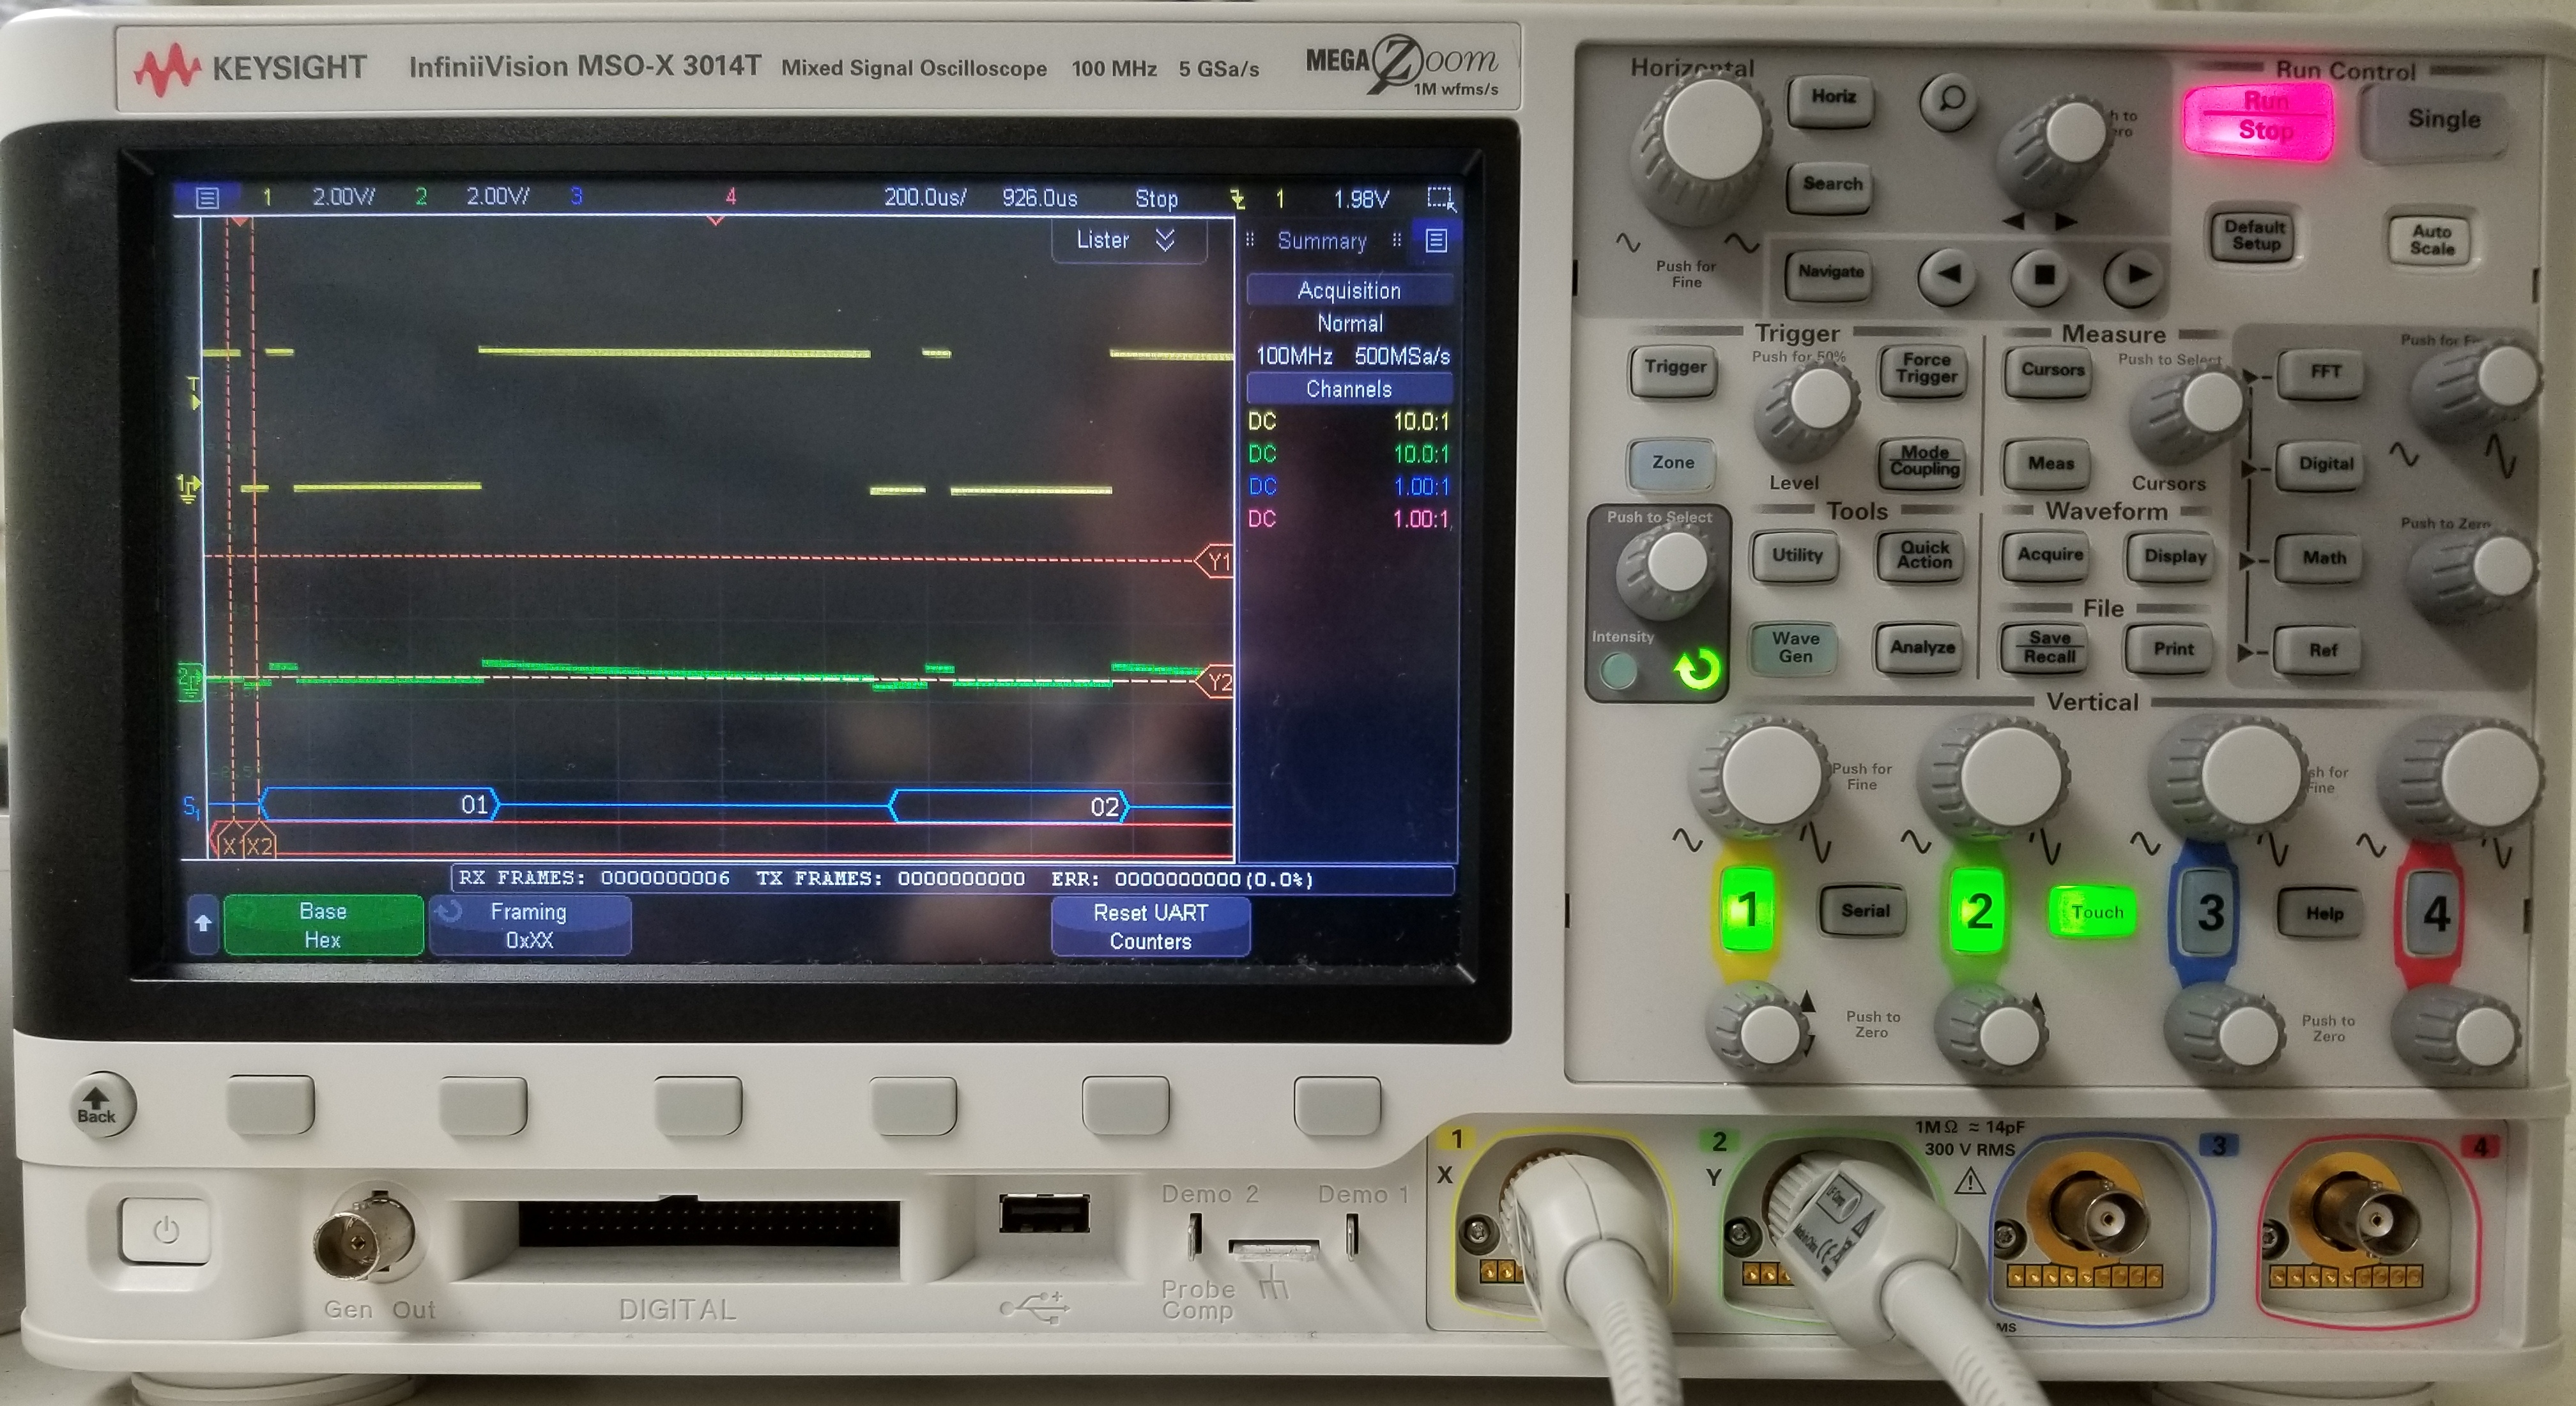
\includegraphics[width=\textwidth]{full_scope}
    \caption{An oscilloscope properly decoding data from a UART bus}
  \end{figure}

  \subsection{Making the Measurement}

  Firstly, the oscilloscope must be turned on and the proper number of probes
  must be connected. For UART, two cables are needed to test two way
  asynchronous communications. If only one signal needs to be decoded, then only
  one cable needs to be connected to the oscilloscope. However, having more
  cables connected to the oscilloscope won't hurt anything, it just clutter up
  your area.

  \begin{wrapfigure}{r}{0.4\textwidth}
    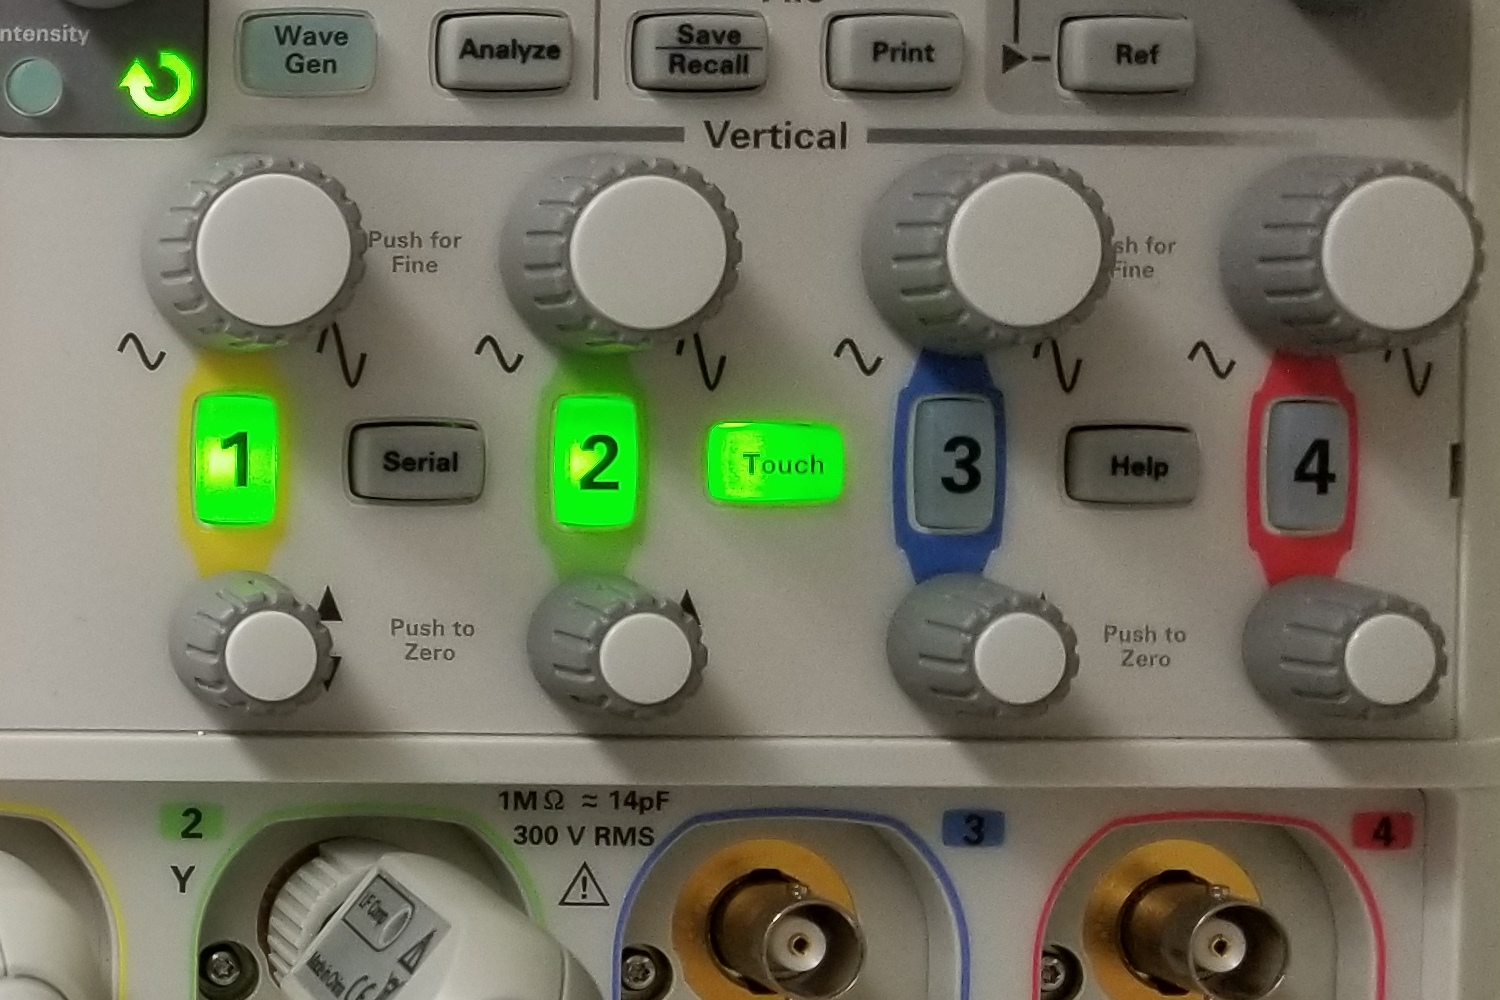
\includegraphics[width=30ex]{serial_button_scope}
    \caption{Serial button located between probe configuration buttons 1 and 2.}
  \end{wrapfigure}

  The oscilloscopes have a Serial button located between buttons 1 and 2.
  Pressing this button opens the serial protocol decoding menu at the bottom of
  the display. Here, settings can be adjusted to match expected bus
  configurations.


  \begin{wrapfigure}{r}{44ex}
    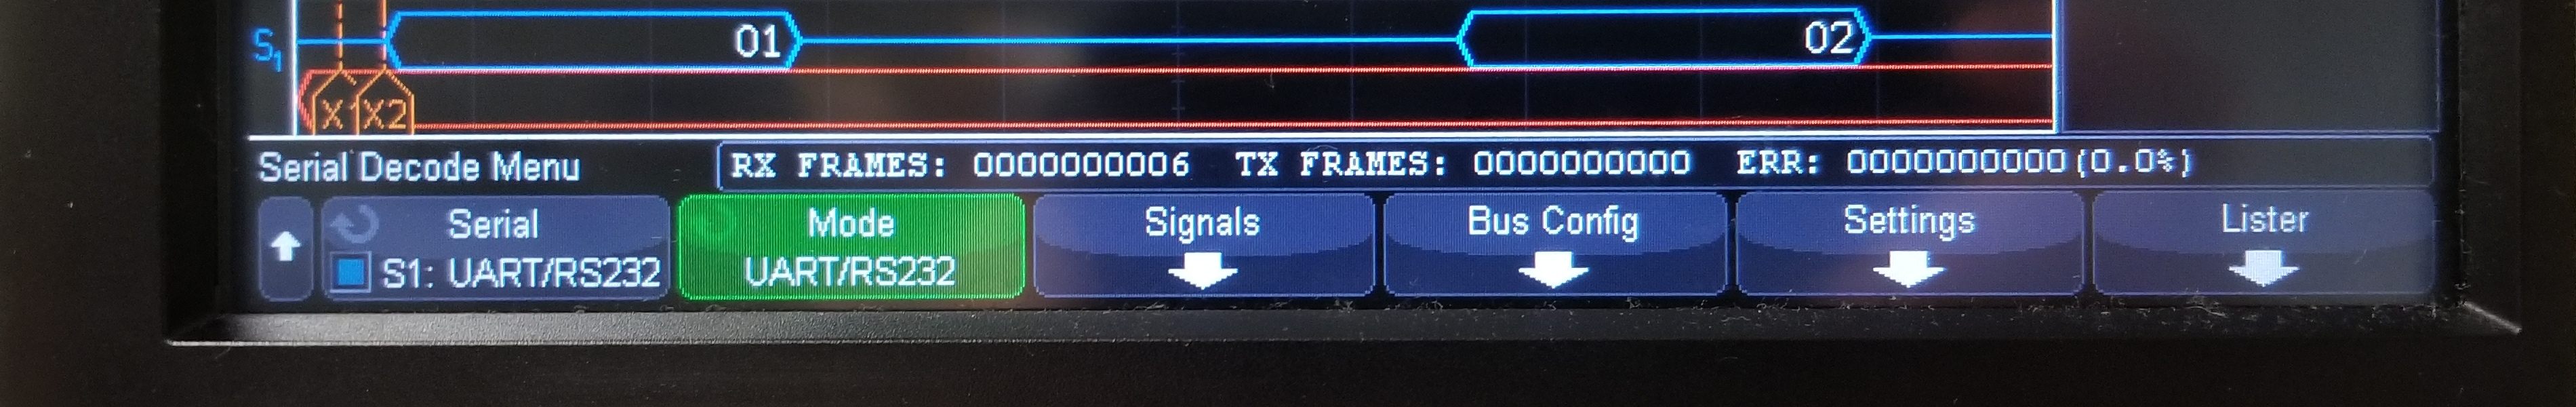
\includegraphics[width=44ex]{serial_decode_scope}
    \caption{Serial Decode Menu. Currently shown with UART/RS232 selected.}
  \end{wrapfigure}

  \begin{wrapfigure}{r}{25ex}
    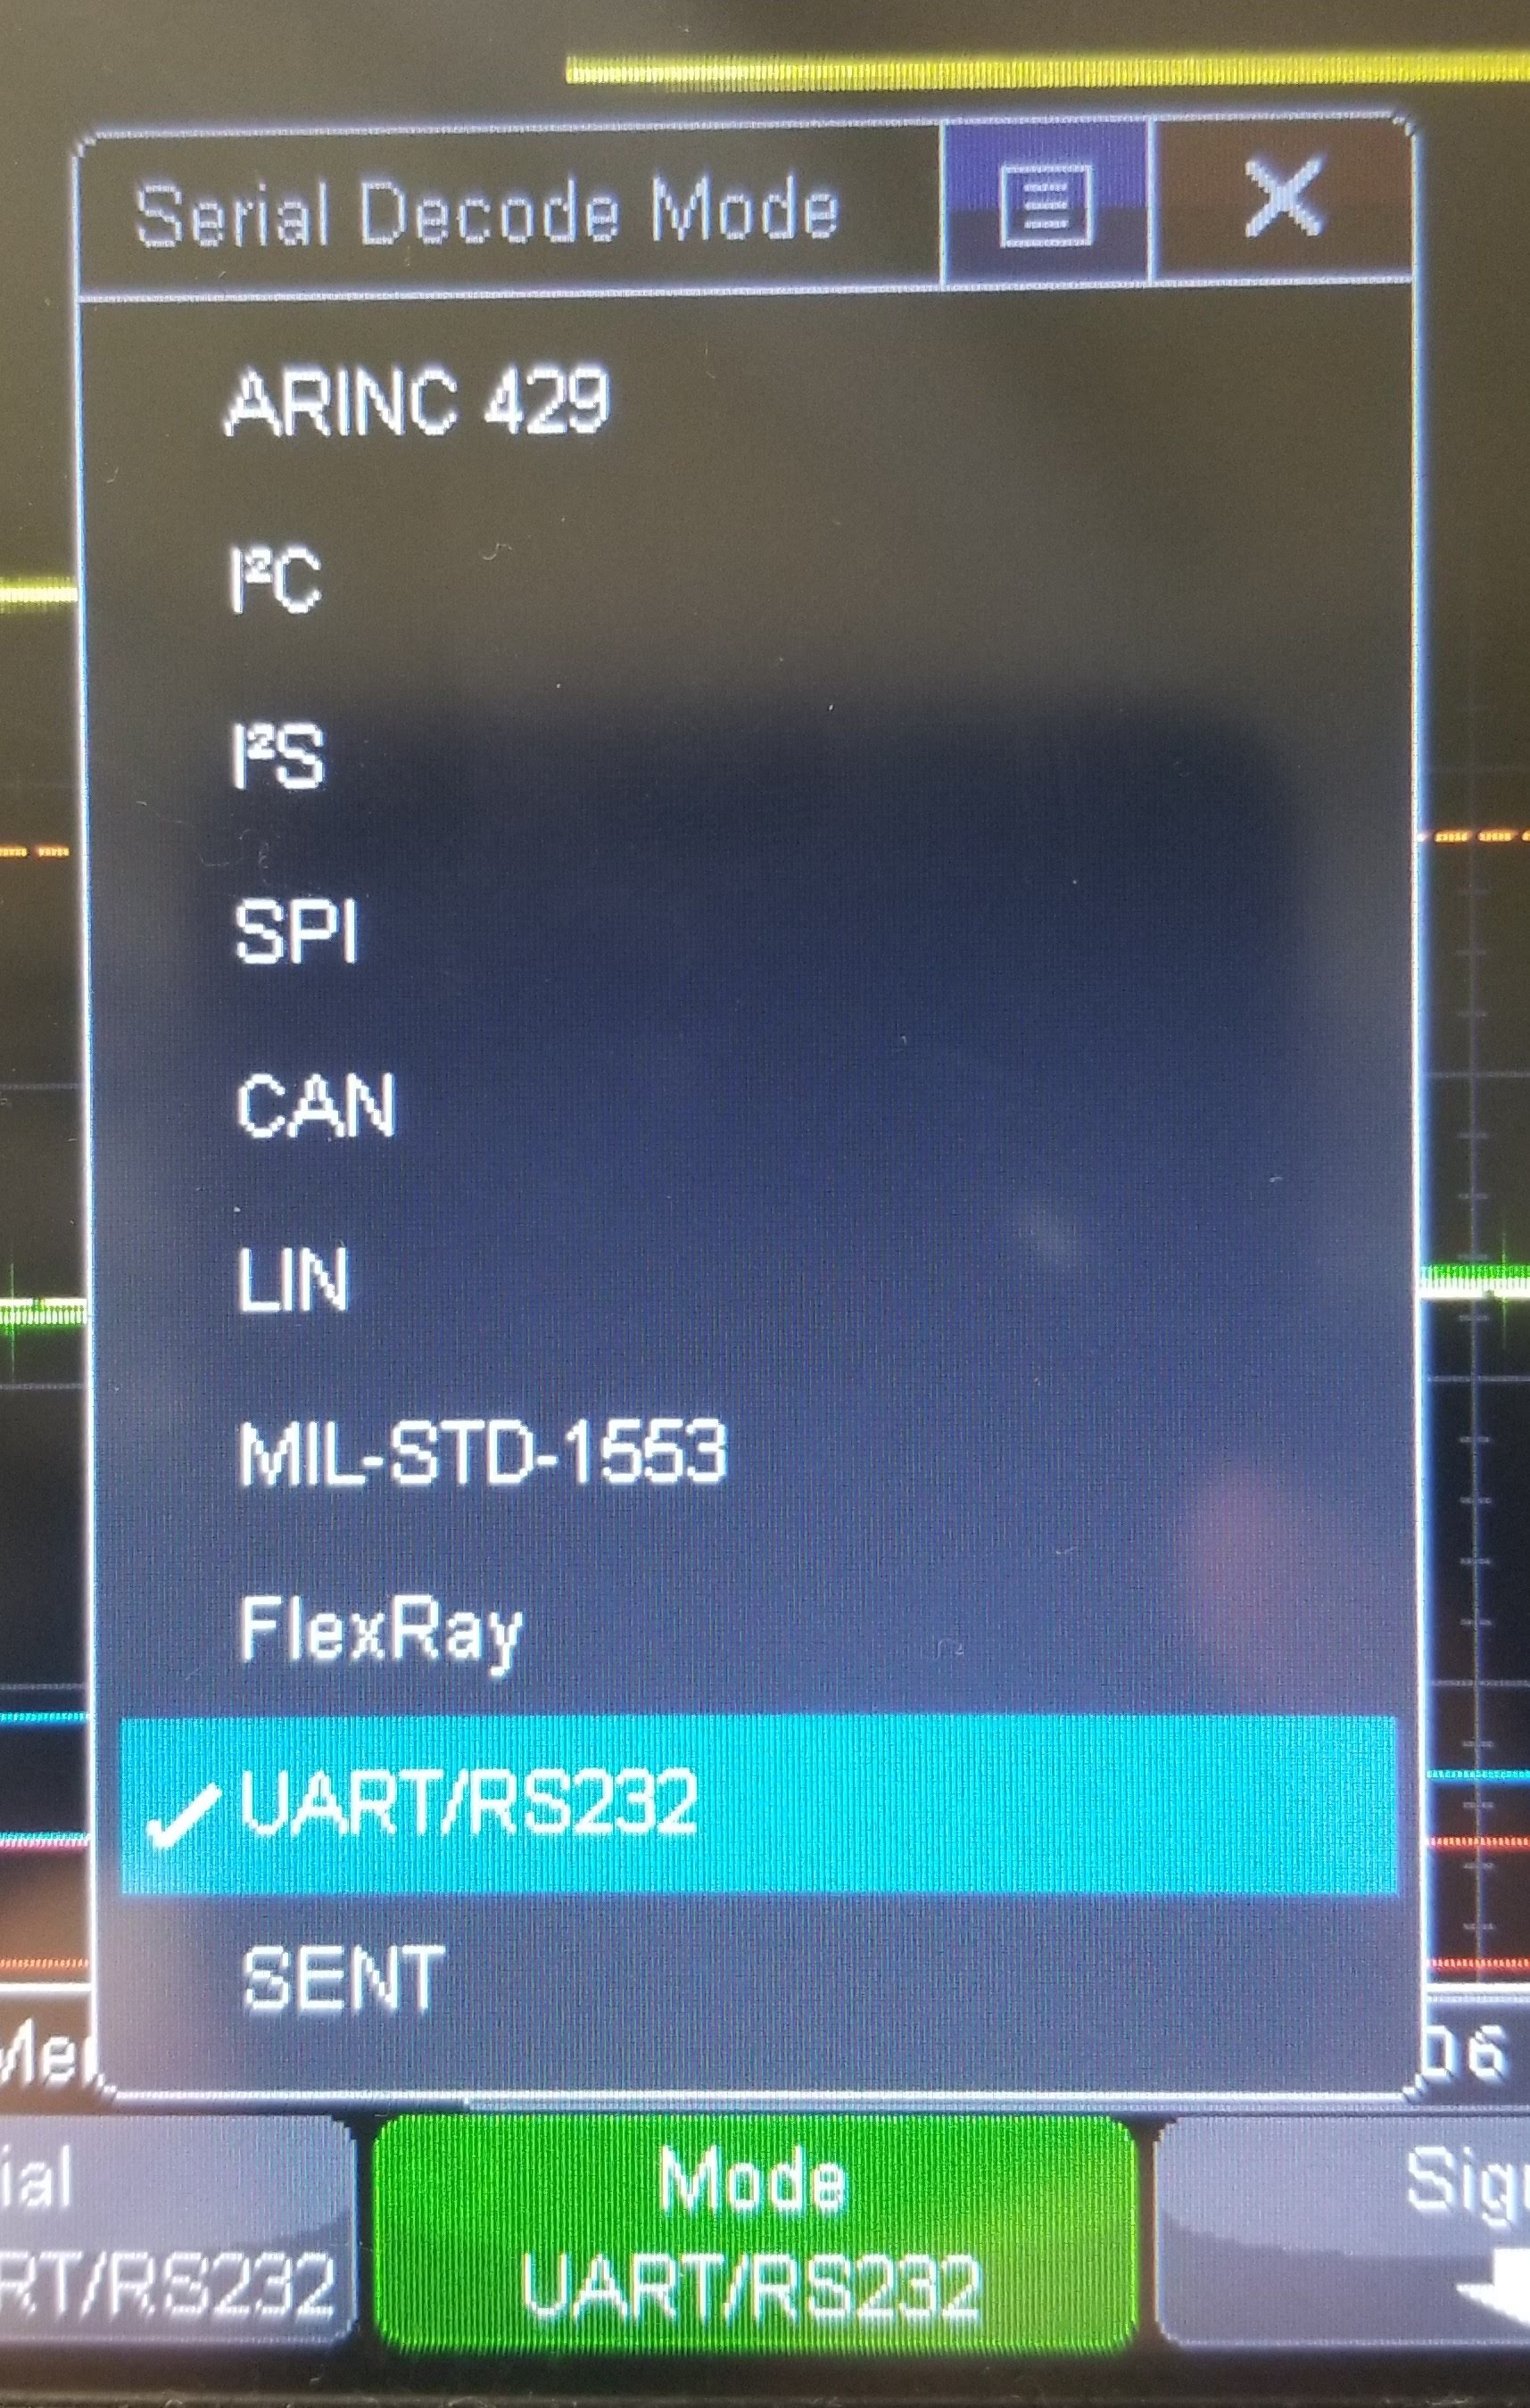
\includegraphics[width=25ex]{mode_menu}
    \caption{Mode selection menu on oscilloscope}
  \end{wrapfigure}

  Inside the menu, selecting the mode button provides a list of communication
  protocols the oscilloscope can decode. This section describes UART decoding,
  so select UART/RS232 from the list. Other sections discuss how to decode some
  of the other protocls listed here. After selcting UART/RS232, the remaining
  entries in the Serial Decode Menu are now specific to decoding UART/RS232.

  % Signals submenu
  The signals submenu gives the ability to specify which input is associated
  with which signal. In the case of UART, the availbalbe signals are Rx and Tx.
  In the example, channel 1 is set to Rx and receives the signals that are
  leaving through the devices Tx connection. The channel could be connected to
  either Rx or Tx from the device, but sticking with convention should help to
  prevent confusion while debugging. The thresholds for signals can also be
  adjusted here in case different voltages are being used. The threshold shown
  % TODO add figure and figure reference
  for Rx was set to just above the threshold for logic high in the device meant
  to receive the signals. The Tx signal was not set because, for this example,
  there was no Tx signal connected. Now that the oscilloscope knows which signal
  is connected to which channel, the bus settings can be configured so signals
  can be properly decoded.

  \begin{figure}[h]
    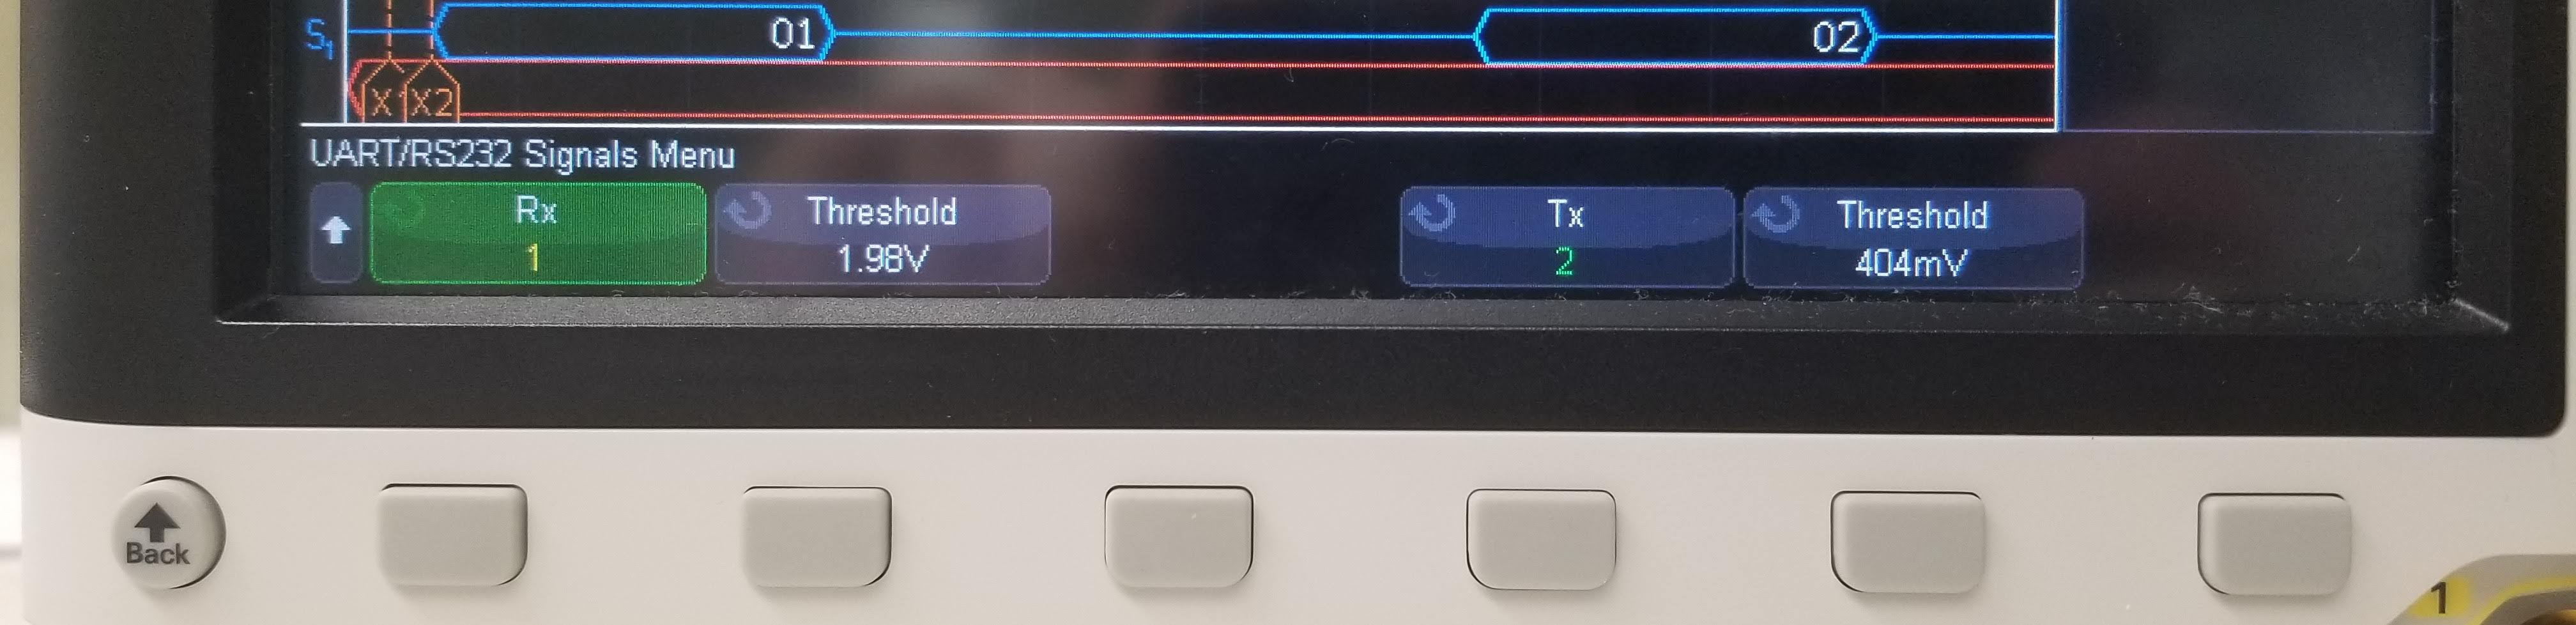
\includegraphics[width=0.7\textwidth]{signals_menu}
    \caption{Signals submenu showing channel 1 as Rx with a threshold of 1.98V}
  \end{figure}

\end{document}
